\subsection{Architektur eines \ac{DBMS}}



\begin{figure}[ht]
  \centering
  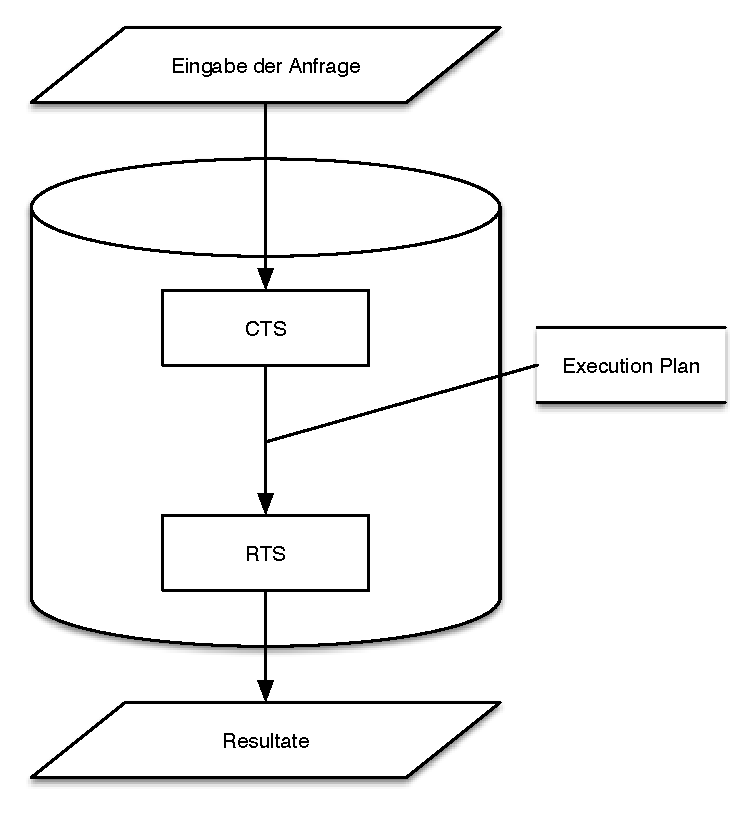
\includegraphics{02_Grundlagen/CTS_RTS.pdf}
  \caption{Architektur eines Datenbanksystems}
  \label{Database_Architecture}
\end{figure}

Die Architektur eines \ac{DBMS} lässt sich in zwei Teile gliedern: \ac{CTS} und \ac{RTS}. Jedes Teilsystem ist für eine andere Aufgabe verantwortlich. Eine Kommunikation beider Elemente findet i.d.R. nur unidirektional statt. Vom \ac{CTS} hin zum \ac{RTS}.

Bei der Bearbeitung eines Nutzerkommandos gibt der Nutzer eine Anfrage zuerst in das \ac{CTS} ein. Das \ac{CTS} ist für die Umwandlung der Anfrage in ein für das \ac{RTS} verständliches Format, beispielsweise einen \ac{QEP}, verantwortlich. Ebenfalls nimmt das \ac{CTS} die Optimierung von Kommandos vor. Sobald die Anfrage an das \ac{RTS} weitergegeben ist, wird das Kommando ausgeführt und das Resultat zurück an den Nutzer übermittelt. Dieser Verlauf ist in Abbildung \ref{Database_Architecture} verdeutlicht.

Es gibt eine Vielzahl an Kommandos, die von einem Nutzer an ein Datenbank-System gestellt werden können. Zu Ihnen zählen neben Anfragen (Queries) beispielsweise auch Indexerstellungen, Schema-  und Datensätzänderungen. Im Folgenden wird das Kommando Anfrage in den Fokus gestellt.

Vor der Verarbeitung muss die Anfrage formuliert werden. Dies geschieht bei relationalen Datenbanksystemen i.d.R. in \ac{SQL}. \ac{SQL} ist eine deklarative Anfragesprache, die sich als Standardsprache für viele Datenbanksysteme durchgesetzt hat. Die fertige Anfrage bildet den Input, der in das Datenbanksystem übergeben wird. 

Eine solche Anfrage kann entweder an ein \ac{QI} oder an ein \ac{QC} System übergeben werden. Ein \ac{QI} ist im Vergleich zu einem \ac{QC} ein einfaches System zur Verarbeitung einer Anfrage. Alle Schritte zur Erzielung eines Ergebnisses werden in einem System ausgeführt. Die Anfrage wird zu diesem Zweck nicht kompiliert, sondern nur interpretiert. Neben Rewriter-Regeln werden keine weiteren Optimierungen durchgeführt. Die Ergebnisse werden direkt an den Nutzer zurückgegeben. Im Gegensatz zu \ac{QI} findet in \ac{QC} Systemen eine komplexere Bearbeitung der Anfrage statt. Dort wird eine Anfrage zuerst in einem \ac{CTS} entgegengenommen, das die Anfrage in einen \ac{QEP} umwandelt, der dann an das \ac{RTS} weitergegeben wird. Im Folgenden werden \ac{QC} genauer behandelt.





\begin{figure}[h]
  \centering
  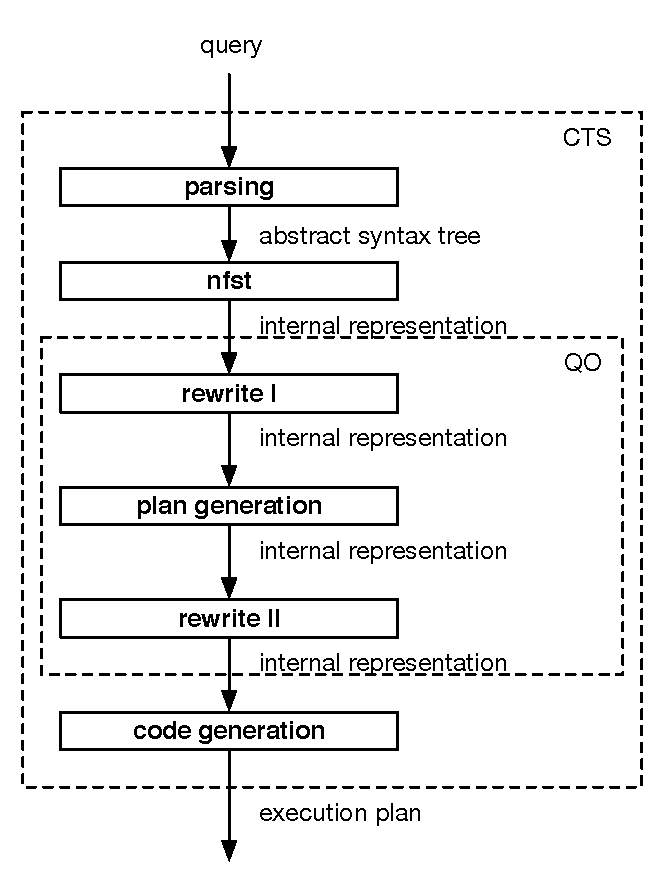
\includegraphics{02_Grundlagen/QCArchitecture.pdf}
  \caption{\ac{QC} Flow}
  \label{DBMS_Interpreter}
\end{figure}


Der \ac{CTS} sieht mehrere Verarbeitungsschritte vor (vgl. Abb. \ref{DBMS_Interpreter}). Zuerst wird die Anfrage in einen abstrakten Syntaxbaum umgewandelt. Dieser Synaxbaum wird mit Hilfe von Normalisierung, Faktorisierung, semantischer Analyse und Übersetzung (nfst) in eine interne Repräsentationsform gebracht. Diese interne Repräsentation wird an den Anfragenoptimierer übergeben, der zuerst mit einem ersten Rewriter die Anfrage einer Bearbeitung unterzieht. Views werden aufgelöst und zusammengeführt, verschachtelte Anfragen werden entschachtelt und neue Prädikate werden abgeleitet. Im nächsten Schritt wird diese veränderte Anfrage an den Plan Generator übergeben. Er ist verantwortlich für das Finden des günstigsten \ac{QEP}. Teil dieser Optimierung ist beispielsweise das Join Ordering. Im letzten Schritt des \ac{QO} wird die Anfrage nochmals durch einen Query Rewriter verändert. Basierend auf diesem Code kann der finale Code generiert werden. Der dem \ac{RTS} als Input für die Ausführung einer Anfrage dient.


Der Plan Generator, der für die Suche nach dem günstigsten Plan verantwortlich ist besteht benötigt, um seine Aufgabe zu erfüllen drei Komponenten \cite{chaudhuri1998overview}: 

\begin{itemize}
\item einen Raum von Plänen (Search Space), aus denen der beste Plan ausgewählt werden kann,
\item einen Enumerator Algorithmus, der für die Suche nach Plänen verantwortlich ist
\item einen Kostenschätzer, der die Kosten für die Ausführung eines jeden Plans abschätzt.
\end{itemize}
